
In this section, the kagome lattices with no magnetic texture $m_0=0$ and with a homogeneous one, as depicted in Fig. \ref{fig: magnetic texture homogenous}, are compared to get an idea where the bands stem from and to illustrate the physical meaning. 
First, we check the sign convention chosen in Eq.~\ref{eq: bloch-Hamiltonian} by using a homogeneous magnetic texture, as depicted in Fig.~\ref{fig: magnetic texture homogenous}. 

\begin{figure}[tbhp]
    \centering
    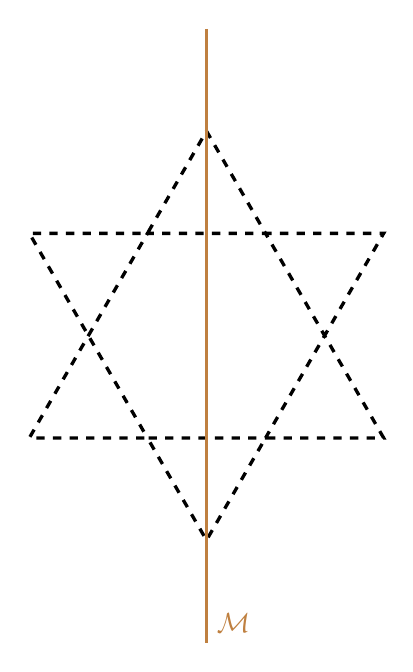
\begin{tikzpicture}[scale=1.5]
    
      % half-length of each spin arrow
      \def\spinhalf{0.3}
    
      % angles of the three sublattices
      \def\phiA{0}
      \def\phiB{0}
      \def\phiC{0}
    
      % useful constants
      \pgfmathsetmacro{\rt}{sqrt(3)}
      \pgfmathsetmacro{\rthalf}{sqrt(3)/2}
    
      % lattice
      \draw[very thick, dashed]
        (0,0) -- (0.5,\rthalf) -- (1.5,\rthalf) -- (2,0)
        -- (1.5,-\rthalf) -- (0.5,-\rthalf) -- (0,0)
        -- (-0.5,\rthalf) -- (0.5,\rthalf) -- (1,\rt)
        -- (1.5,\rthalf) -- (2.5,\rthalf) -- (2,0)
        -- (2.5,-\rthalf) -- (1.5,-\rthalf) -- (1,-\rt)
        -- (0.5,-\rthalf) -- (-0.5,-\rthalf) -- (0,0);
        
        \draw[thick, brown] (1,{3*sqrt(3)/2}) -- (1,{-3*sqrt(3)/2}) node[above right]{$\mathcal{M}$};
      % sublattice A
      \foreach \x/\y in {
        1/{-\rt},
        0/0,
        1/{\rt},
        2/0
      }{
        \centerspin[pastelblue]{(\x,\y)}{\phiA}
      }
    
      % sublattice B
      \foreach \x/\y in {
        0.5/{\rthalf},
        1.5/{-\rthalf},
        -0.5/{-\rthalf},
        2.5/{\rthalf}
      }{
        \centerspin[pastelred]{(\x,\y)}{\phiB}
      }
    
      % sublattice C
      \foreach \x/\y in {
        0.5/{-\rthalf},
        1.5/{\rthalf},
        -0.5/{\rthalf},
        2.5/{-\rthalf}
      }{
        \centerspin[pastelgreen]{(\x,\y)}{\phiC}
      }

    \end{tikzpicture}
    \caption{The homogeneous magnetic texture on a kagome lattice with the mirror symmetry plane $\mathcal{M}$.}
    \label{fig: magnetic texture homogenous}
\end{figure}
Then, by computing the Fermi-surface spin texture for the resulting Hamiltonian in the nonbreathing limit, Fig.~\ref{fig:homogenous-nonbreathing} is obtained. Thus, the spins align parallel for higher energies along the magnetic order, as discussed in Section\ref{section: tightbinding} thereby confirming the introduced sign convention. Note that with SOC the spins acquire additional components, and hence it is possible for them to align antiparallel for higher energies.\\

\begin{figure}[tbhp]
    \centering
    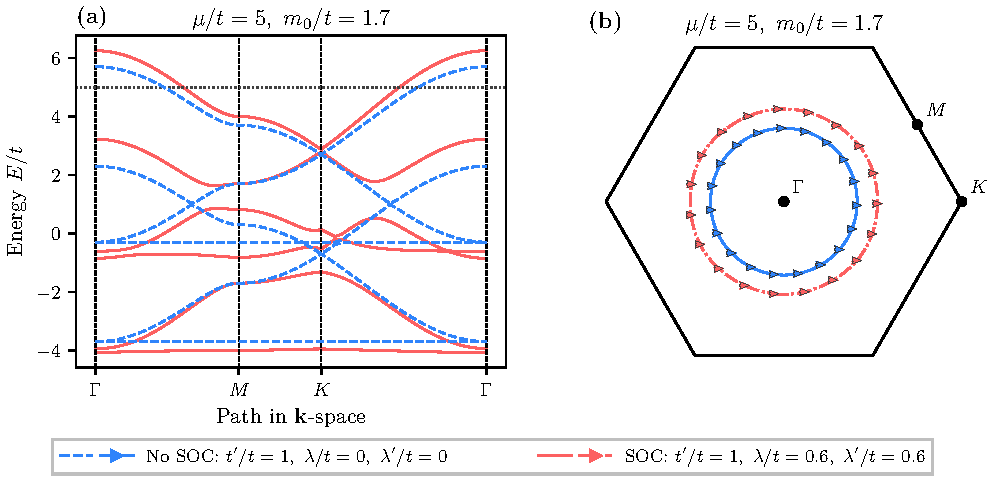
\includegraphics[
        width=\linewidth
    ]{Appendix/homogenous/homogenous_nonbreathing.pdf}
    \caption{\textbf{Results obtained using the tight-binding Hamiltonian \eqref{eq: bloch-Hamiltonian} for the homogeneous magnetic texture, as depicted in Fig. \ref{fig: magnetic texture homogenous} in the nonbreathing limit without and with SOC, respectively.} (a) Band structure along the high-symmetry path $\Gamma$-$K$-$M$, (b) the in-plane Fermi surface spin textures for the chemical potential $\mu$.}
    \label{fig:homogenous-nonbreathing}
\end{figure}

Finally, Fig.~\ref{fig:homogenous-notexture} compares the band structures (a),(b) without a magnetic texture with those for the (c),(d) homogeneous texture. 
For $t'= \lambda = \lambda'=0$, the nonmagnetic kagome lattice has two distinct flat bands, with one of them being orbital degenerate. The flatness stems from the fact that the electrons cannot propagate in the lattice because of a missing hopping on the upward-facing triangles. One might expect three flat bands, however, it can easily be verified by solving the Hamiltonian
\begin{align}
    \mathfrak{H}(\mathbf{k}) = t\begin{pmatrix}
        0&   e^{-i\mathbf{k}\cdot \mathbf{a}_1} &   e^{i\mathbf{k}\cdot \mathbf{a}_3} \\
          e^{i\mathbf{k}\cdot \mathbf{a}_1} & 0 &    e^{-i\mathbf{k}\cdot \mathbf{a}_2} \\
        e^{-i\mathbf{k}\cdot \mathbf{a}_3} &   e^{i\mathbf{k}\cdot \mathbf{a}_2} & 0 
    \end{pmatrix},
\end{align}
following from $\hat{t}_i = t \hat{I}_2$ and $\hat{t}' = t'\hat{I}_2 = 0$ and removing the spin dependence due to a spin-independent Hamiltonian. Solving the matrix with the earlier defined cell-connection vectors $\mathbf{a}_i$, which sum to zero, the eigenvalues $E_+ = 2t$ and the twofold degenerate $E_- = -t$ are obtained. Therefore, the upper band is twofold degenerate and the lower one fourfold degenerate, including an orbital degeneracy. 
Now, by adding SOC with $\lambda'=t'=0$, we obtain three flat bands, occurring due to a broken orbital degeneracy. Note that the bands are still Kramers-degenerate. 

\begin{figure}[tbhp]
    \centering
    \begin{subfigure}[t]{0.85\textwidth}
        \centering
        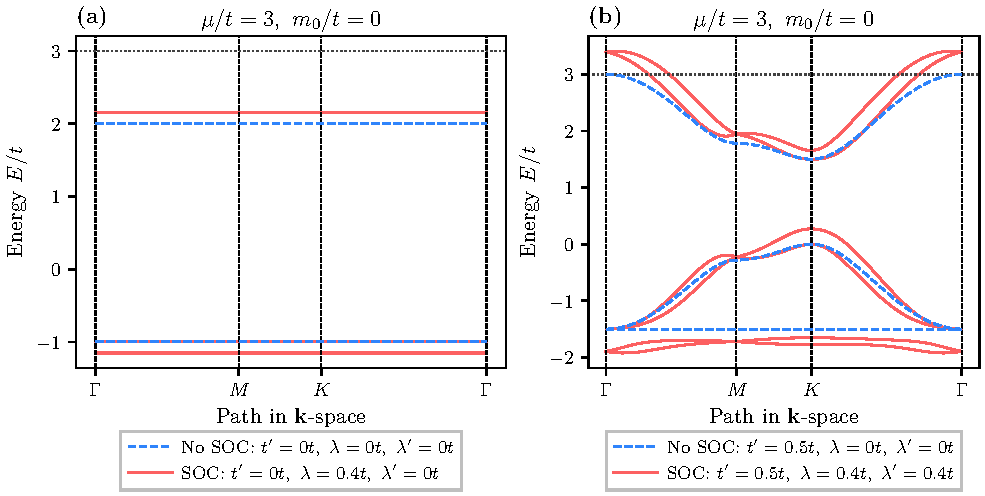
\includegraphics[
            width=\linewidth
        ]{Appendix/no texture vs homogenous/no texture.pdf}
        
    \end{subfigure}
    \vspace{2cm}
    \begin{subfigure}[t]{0.85\textwidth}
        \centering
        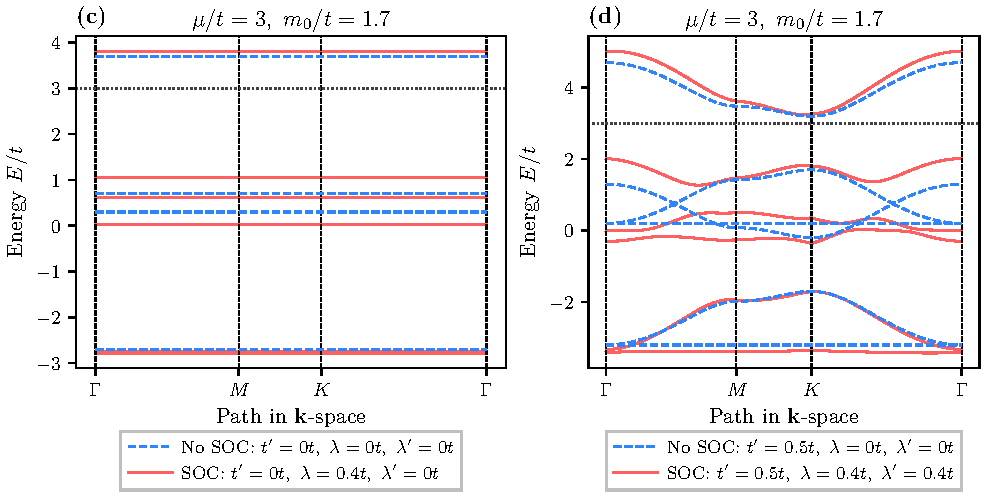
\includegraphics[
            width=\linewidth
        ]{Appendix/no texture vs homogenous/texture.pdf}
        
    \end{subfigure}
    \caption{\textbf{The computed band structure along the high-symmetry path $\Gamma$-$K$-$M$ for the Hamiltonian in Eq.~\eqref{eq: bloch-Hamiltonian}.} Results for no magnetic texture (a) without SOC, (b) with SOC and for an homogeneous magnetic texture, depicted in Fig.~\ref{fig: magnetic texture homogenous}, (c) without SOC and (d) with SOC.}
    \label{fig:homogenous-notexture}
\end{figure}

By adding a magnetic texture, the Kramers degeneracy is broken and therefore there are twice as many distinct bands, due to the magnetic texture breaking time-reversal and the lack of an antiunitary symmetry protecting the degeneracy.

Furthermore, by adding hopping on upward-facing triangles, so $t'\neq0$ or $\lambda'\neq 0$, dispersive bands are obtained, as seen in Fig.~\ref{fig:homogenous-notexture} (b), (d). For no SOC and no magnetic texture, Kramers pairs are expected, resulting in three twofold degenerate bands, as observed.  These bands are split by adding SOC or a magnetic texture, therefore resulting in six dispersive bands.
In the absence of SOC for a breathing lattice, it is interesting to note that there still exists a twofold degenerate flat band for no magnetic texture, or a flat band for the magnetic lattice. This arises from the lattice and magnetic geometry, leading to destructive interference. A detailed analysis of this flat band is beyond the scope of this work.
None of the not-treated cases, for example breathing lattice with SOC, are not analyzed in detail because we expect up to six dispersive bands in all of them, where degeneracies, forced by the lattice and magnetic geometry may occur. 




